% !TEX root = ../../../main.tex
%

\newpage
\section{Progettazione}
\subsection{Tipo di presa}

\begin{wrapfigure}{r}{5cm}
  \centering
  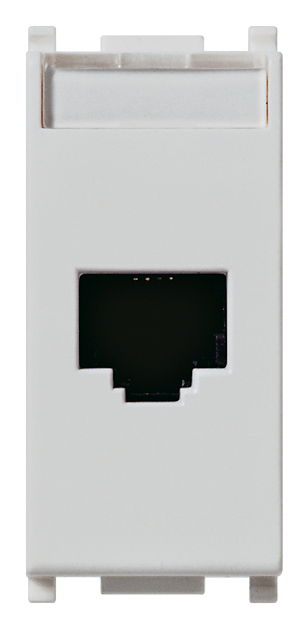
\includegraphics{vimar-14338-8-SL.jpg}
  \caption{Il connettore scelto per le prese utente.}\label{fig:presa}
\end{wrapfigure}

Supponendo che l'edificio abbia già alcune scatole elettriche incassate dedicate all'impianto di rete,
dove necessarie (anche condivise con altri connettori/controlli), non si terrà conto del costo di queste ultime.

Si sceglie di utilizzare prodotti di marca Vimar, serie Netsafe.
Nello specifico, si sceglie di usare dei connettori RJ45 Cat5e UTP (codice 14338.8.SL), illustrato in figura~\ref{fig:presa}.

Dato che determinate scatole elettriche possono contenere anche prese, pulsanti, interruttori o altri tipi
di dispositivi, non si conosce la dimensione (e di conseguenza il costo) delle placche decorative e dei supporti di montaggio.

Si suppone pertanto di affidarsi a quanto già predisposto per l'impianto elettrico (ove possibile).

Notare che nella maggior parte dei casi, questo non sarà necessario, in quanto gran parte dell'impianto,
per motivi di flessibilità e semplicità, verrà posato a pavimento, con delle prese direttamente disponibili sulle scrivanie.

Nei casi in cui è invece necessario affidarsi a delle prese a muro, resta valido quanto prima descritto.

\subsection{Dislocazione degli armadi e dorsale principale}

Data la topografia stellare del cablaggio orizzontale, si preferisce ospitare gli armadi per la \textit{floor distribution}
nei locali tecnici centrali all'edificio, in ogni piano. Essendo già stato fissato dalla planimetria fornita, il centralino
telefonico sarà per forza posizionato nel locale tecnico sud-ovest del piano terreno, assieme alle apparecchiature per
il collegamento alla rete pubblica.

Con questa scelta, il server (posizionato al piano terreno), godrà di una distanza ridotta con l'armadio di piano, garantendo
un miglior collegamento (in quanto si assume che il server necessiti di una considerevole quantità di banda), ed una maggiore
flessibilità nel caso in cui, in futuro, dovessero essere necessarie delle espansioni.

I collegamenti di dorsale dell'edificio saranno inizialmente orizzontali, dirette dal locale tecnico sud-ovest del piano terreno
verso quello centrale. Da quel punto, si muoveranno in verticale, raggiungendo gli altri armadi. La stessa cosa vale per i collegamenti
addizionali tra armadi adiacenti.

\subsection{Cablaggio orizzontale}

Si suppone di avere a disposizione un sistema di cablaggio a pavimento galleggiante, comprensivo di più canalette di larghezza sufficientemente
ampia da poter accogliere complessivamente, nelle parti iniziali del percorso, circa la metà di tutti i cavi utilizzati nel cablaggio di un singolo piano.

Per quanto concerne la sala riunioni, essendo adiacente al locale tecnico contenente l'armadio, ed essendo dotata di numerose prese,
si preferisce evitare di dover passare il cablaggio attraverso il corridoio: si preferisce attraversare il muro, predisposto con
un foro di diametro sufficiente, per raggiungere i tavoli da sotto il pavimento. Qui, le connessioni saranno poste al centro del tavolo principale
e su quello del presentatore mediante delle scatole elettriche oblique da scrivania.

Si ritiene utile sfruttare un passaggio simile per il raggiungimento della vicina sala server e, per i piani superiori,
del corridoio al lato opposto della porta presente nel locale tecnico. Non si ritiene ragionevole la percorrenza a ``U'' del corridoio
principale per il solo fine di raggiungere degli uffici altrimenti molto vicini in linea d'aria.

Queste considerazioni sono riportate nelle planimetrie di fine capitolo (figure~\ref{fig:planimetria-terreno-cablaggio}~e~\ref{fig:planimetria-1-cablaggio}). I cablaggi di dorsale sono tracciati con delle linee
di spessore maggiore, ed i cerchi indicano il passaggio tra piani differenti.

Gli armadi sono evidenziati in azzurro e le prese in fuchsia.

\begin{figure}[ht]
  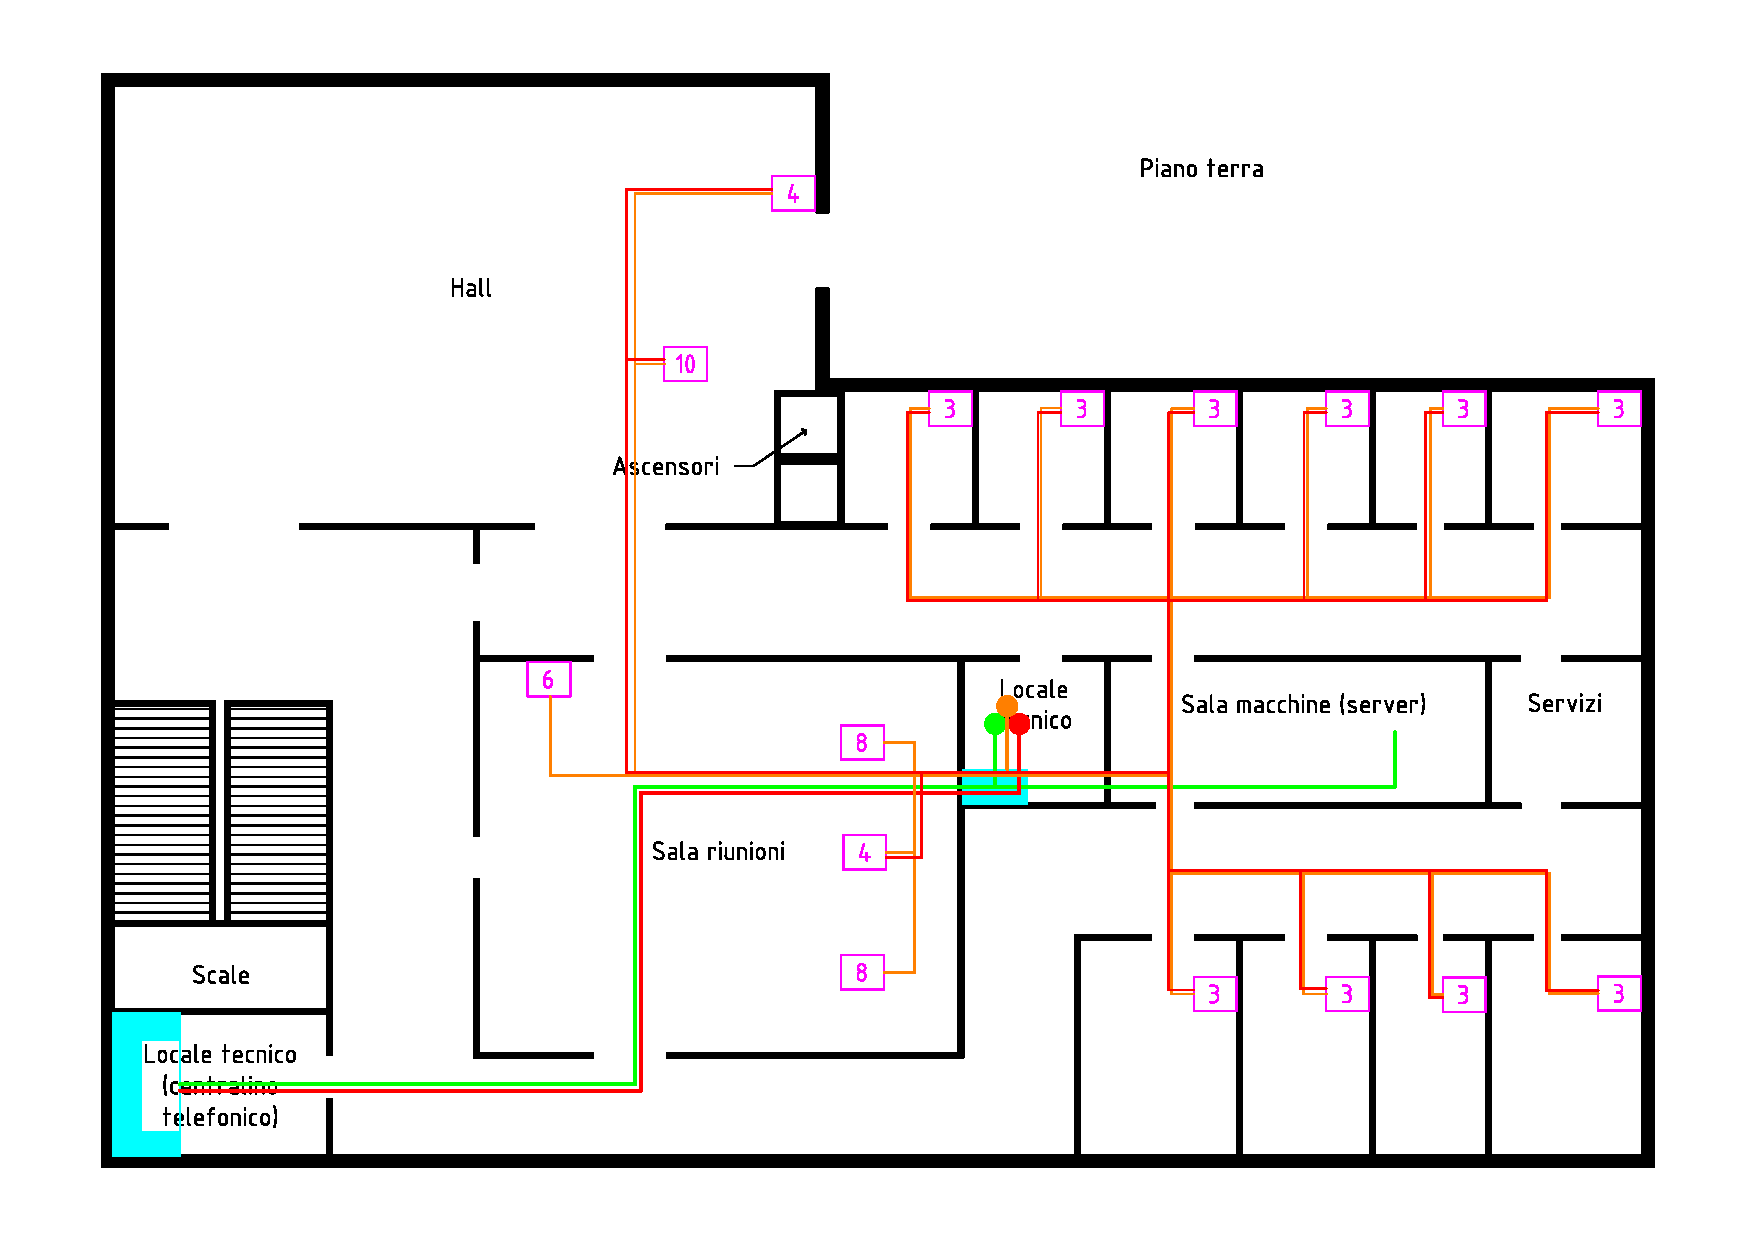
\includegraphics[angle=90,origin=c,width=\textwidth]{planimetrie-pianoterra-cablaggio}
  \caption{Cablaggio del piano terreno.}\label{fig:planimetria-terreno-cablaggio}
\end{figure}

\begin{figure}[ht]
  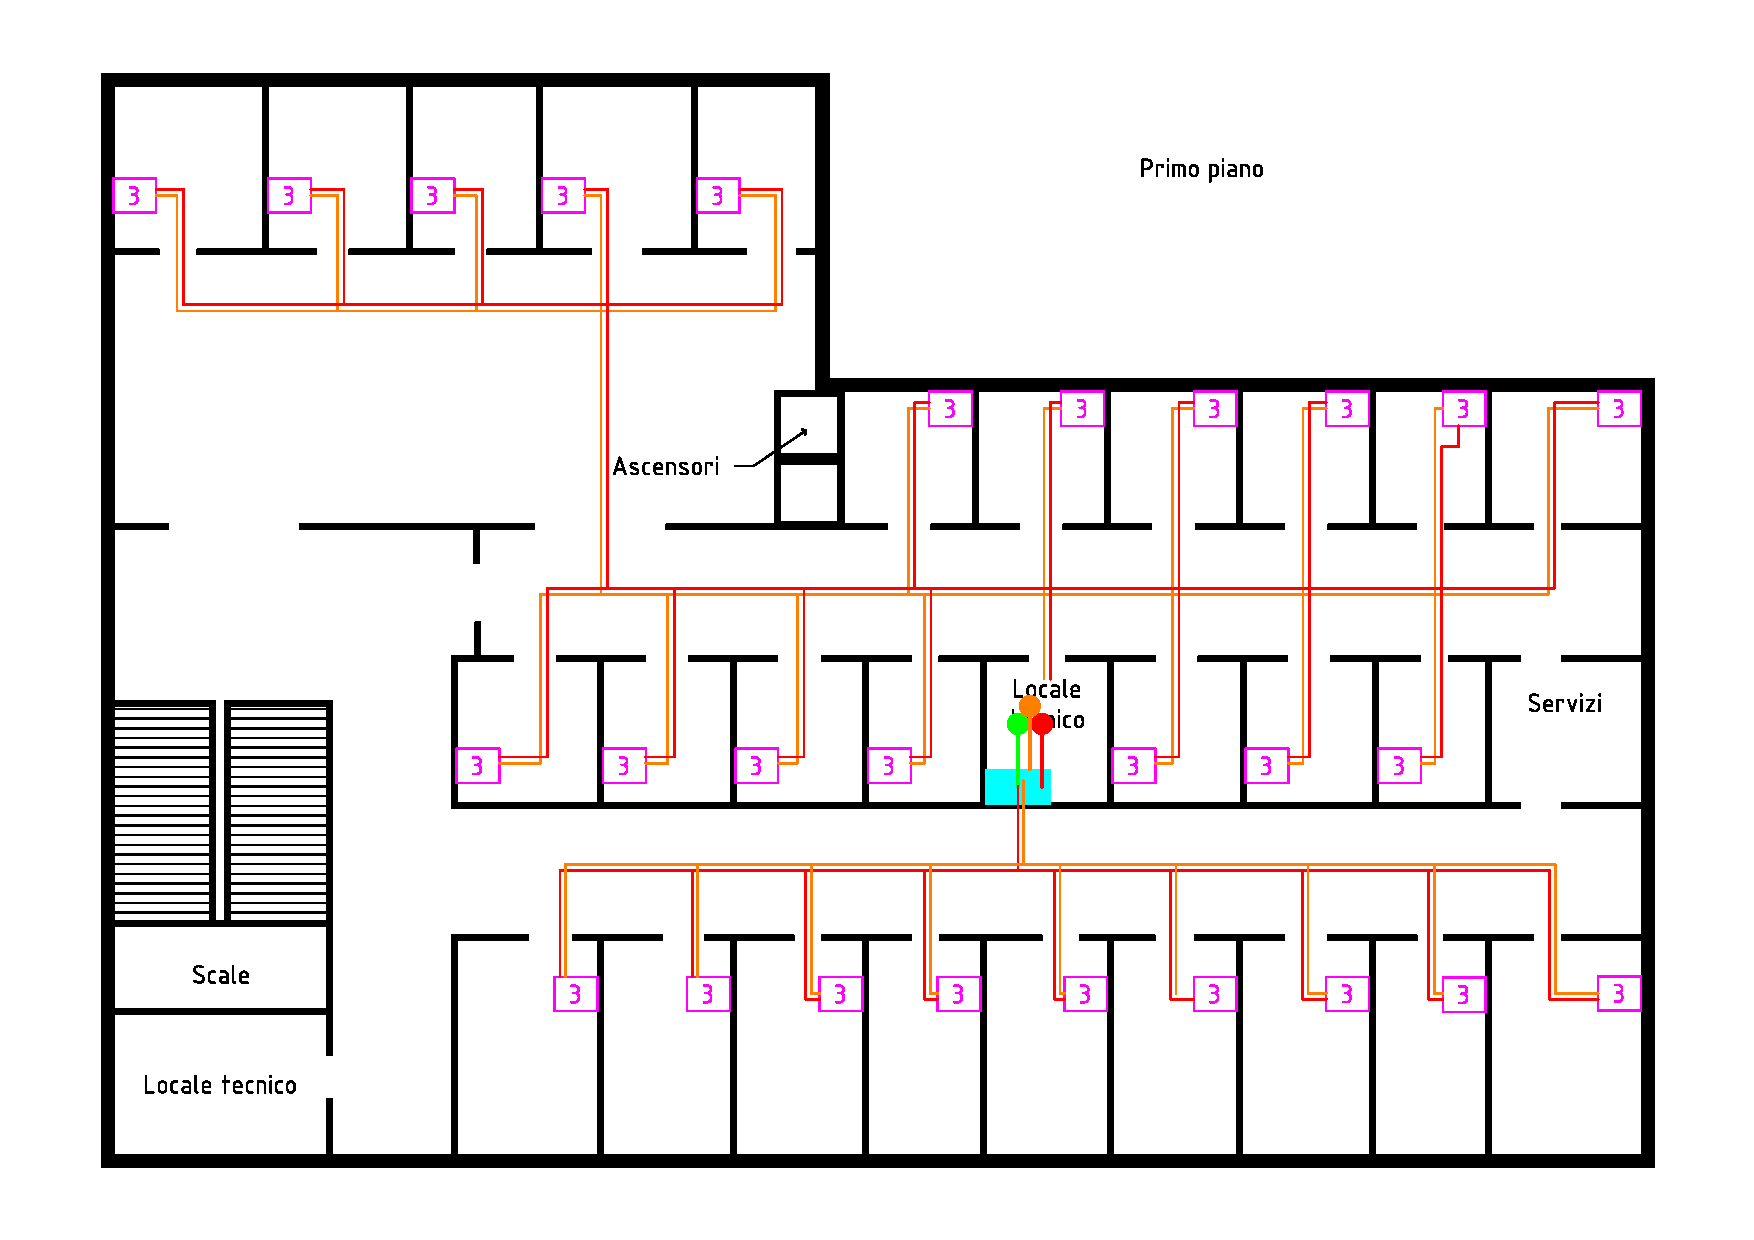
\includegraphics[angle=90,origin=c,width=\textwidth]{planimetrie-piano1-cablaggio}
  \caption{Cablaggio dei piani da primo a quarto.}\label{fig:planimetria-1-cablaggio}
\end{figure}

Nelle planimetrie, il cablaggio si distingue nel seguente modo:
\begin{description}
  \item[Verde] Fibra ottica multimodale 50/125.
  \item[Arancione] Cavi in rame Cat5e per Ethernet.
  \item[Rosso] Cavi in rame voice-grade (Cat3) per fonia.
\end{description}

Si contano due pareti attraversate nel piano terra, e soltanto una per piano nei superiori.

\subsection{Armadio del piano terreno}
L'armadio del piano terreno è quello direttamente connesso al centralino telefonico ed ai sistemi di collegamento con
l'infrastruttura di rete pubblica.

In questo armadio sarà presente sia il \textit{floor distributor} per il pianterreno, sia il \textit{building distributor}.
Volendo, possono essere separati per avere una migliore suddivisione, ma vista la minor densità del piano terreno rispetto
ai superiori, si ritiene più comodo l'utilizzo di un unico armadio.

Per poter definire il numero di prese nei pannelli di permutazione, è necessario stabilire il livello di ridondanza anche
nei collegamenti di dorsale.

Si decide di utilizzare un cavo da 12 fibre ottiche (Vimar 03152.E) per il collegamento dei \textit{floor distributor} con il \textit{building distributor}.
Per il collegamento tra il centralino telefonico (punto di connessione con l'esterno anche per la fibra ottica) ed il locale tecnico
si ritiene utile l'uso un cavo da 4 fibre (Vimar 03153.E). Soltanto due di queste saranno utilizzate, ma essendo la parte più delicata della rete, è il
primo luogo in cui è necessario garantire una buona ridondanza. La commutazione sulla linea secondaria deve essere estremamente rapida e non
deve richiedere interventi da parte di esterni in caso di guasto.

\newpage
\subsubsection{Pannello di permutazione per fibra ottica}
\begin{wrapfigure}{r}{7cm}
  \centering
  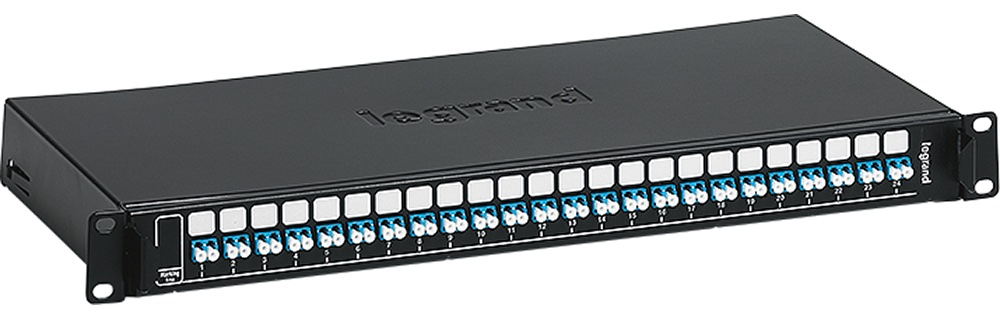
\includegraphics[width=7cm]{BTI_C9124LCL.jpg}
  \caption{Il pannello di permutazione per fibra ottica.}\label{fig:patch-panel-fibra}
  \vspace{-1.5cm}
\end{wrapfigure}
È necessaria una striscia di permutazione per fibra ottica con capacità minima di 6 coppie.
Il \textit{patch panel} scelto è il Bticino/Legrand C9124LCL, dotato di connettori LC, 48 fibre, multimodale,
con montaggio a rack.

\subsubsection{Pannelli di permutazione telefonica}
Il \textit{building distributor} è predisposto per poter permutare tutte le utenze telefoniche prima del loro
arrivo ai \textit{floor distributors}. Essendoci un totale di 122 utenze telefoniche interne e garantendo una
certa espandibilità e ridondanza, si sceglie di usare 4 coppie di pannelli (quattro diretti al centralino, ed
altri quattro dedicati ai singoli piani) di marca Vimar, modello 03024.3. Questi sono dotati di 50 porte RJ45
voice-grade ciascuno (esempio in figura~\ref{fig:patch-panel-fonia}). In questo modo vengono garantiti 200 collegamenti.

\subsection{Parti comuni a tutti gli armadi}
In ogni armadio, arrivano i seguenti collegamenti:
\begin{enumerate}
  \item Un numero piuttosto elevato di collegamenti telefonici verso il centralino.
  \item Una coppia di fibre ottiche, connesse con il permutatore ottico di centro stella (BD).
  \item I collegamenti di backup tra locali tecnici adiacenti.
\end{enumerate}

\begin{wrapfigure}{l}{7cm}
  \centering
  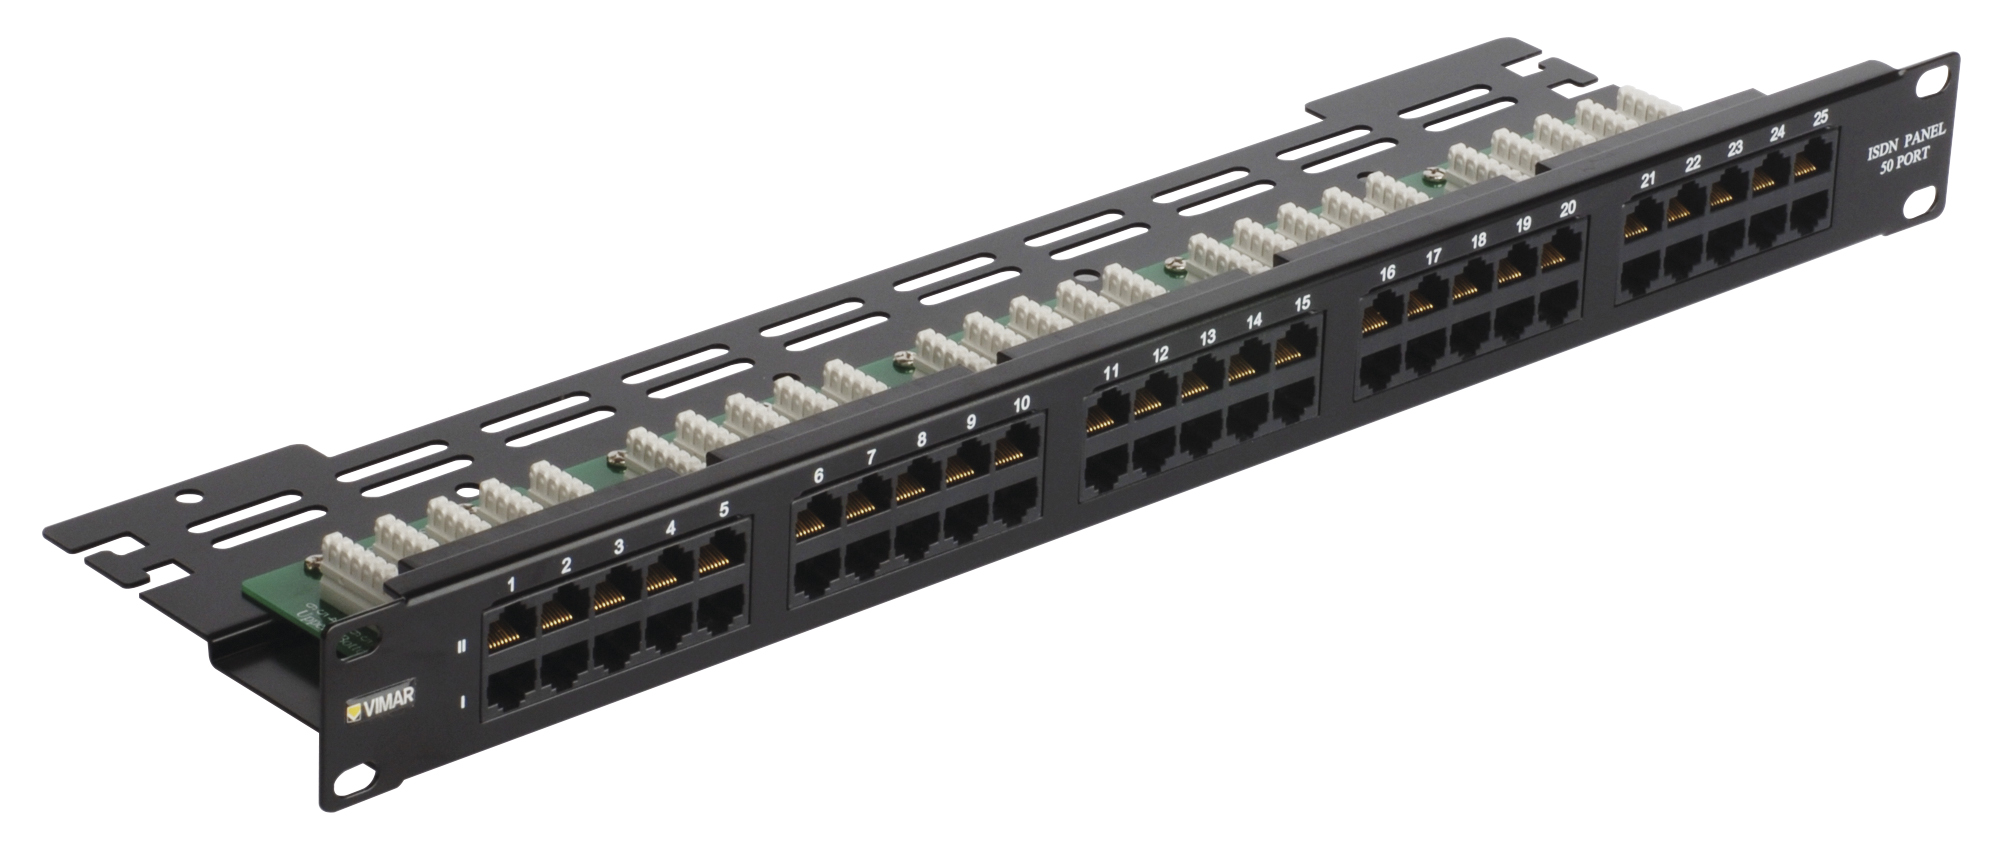
\includegraphics[width=7cm]{vimar-03024-3.jpg}
  \caption{Il pannello di permutazione telefonico.}\label{fig:patch-panel-fonia}
  \vspace{-1cm}
\end{wrapfigure}

Saranno necessarie due strisce di permutazione: una telefonica, connessa al centralino al piano terreno,
ed un'altra di distribuzione verso tutte le prese del piano. Quest'ultima sarà collegata, mediante delle patch-cord,
sia con le prese degli switch di piano, sia con quella telefonica precedentemente indicata.

\subsubsection{Pannello di permutazione telefonico}
Visto che il numero massimo di utenze telefoniche per piano si aggira intorno alle 30 unità,
si decide di utilizzare delle strisce di permutazione Vimar modello 03024.3, 50 prese RJ45 voice-grade,
illustrato in figura~\ref{fig:patch-panel-fonia}.
\begin{wrapfigure}{r}{7cm}
  \vspace{3cm}
  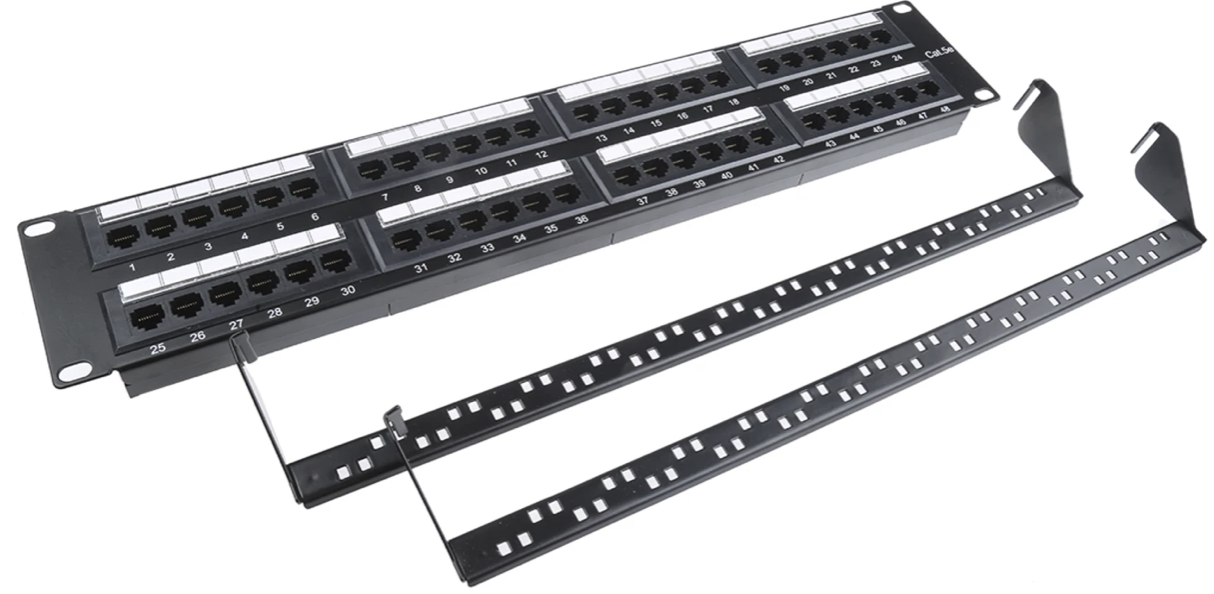
\includegraphics[width=7cm]{rs-pro-556-708.png}
  \caption{Il pannello di permutazione di distribuzione.}\label{fig:patch-panel-distribuzione}
  \vspace{-2cm}
\end{wrapfigure}

\subsubsection{Pannello di distribuzione}
Ogni presa utente del piano andrà connessa a questi pannelli di permutazione. Come prima conteggiato,
il numero massimo di prese per piano è di 81 unità. Si sceglie di utilizzare due \textit{patch panel} di marca
RS Pro, codice 556-708 (Cat5e, 48 porte, RJ45, UTP, 2U, illustrato in figura~\ref{fig:patch-panel-distribuzione})
in ogni \textit{floor distributor}.

\subsection{Cavi}
Si effettua un conteggio approssimativo della quantità di cavi da utilizzare per la realizzazione dell'impianto.

\subsubsection{Collegamento in fibra ottica}
Ha una lunghezza approssimativa di 40 metri. Se si ritiene necessario collegare il server aziendale allo stesso
modo, è ragionevole aggiungere altri 15 metri. Si tratta di un cavo da 4 fibre multimodali 50/125 OM3 (Vimar 03153.E).
Si suppone che l'internet service provider abbia fornito la necessaria attrezzatura per il collegamento fino al
locale tecnico sud-ovest, assieme ai servizi telefonici.

\subsubsection{Dorsale in fibra ottica}
Considerando un'altezza di 3 metri per piano, e tenendo conto del fatto che non si tratterà di un percorso totalmente
rettilineo, si ritiene ragionevole supporre che la dorsale abbia una lunghezza di circa 25 metri. Si sceglie, come
precedentemente indicato, di utilizzare una fibra multimodale 50/125 OM2 (Vimar 03152.E). Il cavo contiene 6 coppie, ed ognuna verrà estratta
dal cavo nel punto in cui è richiesto il collegamento con le apparecchiature attive di rete.

\subsubsection{Collegamento e dorsale telefonica}
Per il collegamento del \textit{BD} con il centralino telefonico, si utilizzerà un cavo in rame multicoppia di categoria 3.
Per coerenza col numero di prese per piano, si sceglie un cavo da 50 coppie, prodotto da Draka Prysmian.
Questo cavo sarà utilizzato sia per collegare il centralino ed il \textit{building distributor}, sia quest'ultimo con gli armadi
di piano. La quantità necessaria di cavo è di 160 metri (4 cavi su 40 metri) per il primo collegamento, ed altri
60-70 metri (garantendo sempre una certa abbondanza) per il cablaggio verticale.

\subsubsection{Cavi per la distribuzione}
Per la distribuzione dei servizi di telefonia ed internet fino agli uffici, si utilizzano cavi di categoria 5e da 4 coppie ciascuno.
Anche le prese ridondanti, previste in ogni ufficio, saranno cablate in questo modo.

La stima di cavo necessario per il piano terreno è di poco inferiore ai 2000 metri (approssimativamente 1750).
Per i piani successivi, questo numero sale a circa 2800 metri. Si decide di considerare un totale di 3000 metri per piano.
A questo scopo, saranno necessari 14000 metri di cavo Cat5e da 4 coppie, UTP.

Considerando la volontà di aggiungere una linea di backup tra armadi adiacenti, composta da 4 cavi, occorre aggiungere cavo sufficiente
a coprire 4 volte la dorsale. Si aggiungono altri 300 metri al conteggio. In questo modo sarà possibile, con il cavo aggiuntivo,
creare dei cavi Ethernet su misura ove necessario.

Si acquisti un totale di almeno 14300 metri di cavo.

Acquistando 14 rotoli di Vimar 03050.E.B (1000 metri) ed un rotolo di 03050.E (305 metri), si giunge a 14305 metri di cavo.